\chapter{METHODOLOGY}
\pagestyle{fancy}

In this chapter, we introduce the proposed model in details. The following parts of this chapter is organized as follows: Section 3.1 formulates the problem and presents nomenclature. In section 3.2, we briefly present the dataset and preprocessing procedure of airport delay features. Finally, section 3.3 introduces the graph-based model and its extensive use case.

\section{Problem Statement}
\label{ch_3_1}

Before formally illustrating the proposed ADMoN model, we make the following nomenclature.
\begin{itemize}
    \item $\mathcal{G}$ A graph consisting of nodes and edges.
    \item $\mathcal{V}$ The set of nodes in a graph.
    \item $v_i$ A node feature vector.
    \item $\mathcal{E}$ The set of edges in a graph.
    \item $e_{ij}$ An edge pointing from $v_i$ to $v_j$.
    \item $A$ The adjacency matrix corresponding to the edge set.
    \item $a_{ij}$ A real-value weight associated to the edge pointing from $v_i$ to $v_j$.
    \item $D$ The diagonal degree matrix.
    \item $L$ The combinatorial graph Laplacian matrix.
\end{itemize}

We consider airport delays mutually affect the origin and destination airport; the relationship is bidirectional rather than unidirectional. Therefore, we model airport delay pattern connections as an undirected graph $\mathcal{G}=(\mathcal{V},\mathcal{E})$ with each node $v_i\in\mathcal{V}$ associated with an individual airport and each edge $e=(v_i, v_j)\in\mathcal{E}$ representing the binding of any two airports.

Intuitively, it's reasonable to presume airports spatially close to each other to have strong binding for sharing similar weather conditions. Airports with high numbers of intra-flights can also have strong binding since the delay of one airport can propagate to the other. However, the former leads to a dense adjacency matrix, leading to cluster collapse. The latter cannot capture the connections related to other factors, for example, local extreme weather. Instead of defining the airport connections as a priori, the proposed model allows the model to extrapolate latent binding based on delay features by integrating a learn-able adjacency matrix $A$.

Suppose we are looking into an airport network of $n$ airports with delay feature of each airport represented as a $d$-dimensional vector $v_i\in\mathbb{R}^d$, the node set is then a matrix $\mathcal{V}=[v_1,\ldots,v_n]^\intercal\in\mathbb{R}^{n\times d}$. The objective of our model is to learn the adjacency matrix that
\begin{itemize}
    \item promotes smooth graph signal;
    \item best fit the properties of an adjacency matrix;
\end{itemize}
and a graph cluster assignments calculated using a semi-specific permute invariant kernel function $C=\text{Softmax}(\mathcal{K}(\mathcal{V}, A))$ that
\begin{itemize}
    \item minimize the average conductance among clusters;
    \item maximize the modularity of the network.
\end{itemize}

If we denote the total estimation loss effect by a function $\mathcal{L}(A,C)$. the objective of our model can be expressed by
\begin{equation}
    A^*, C^* = \underset{A, C}{\text{argmin}}\mathcal{L}(A, C): C=\text{Softmax}(\mathcal{K}(\mathcal{V}, A))
\end{equation}

\section{Data Processing}
Based on the previous studies, flight delay data can contain either flight-level, airport-level, or NAS-level delays\cite{dai2021having}. In our project, ASPM flight level datasets are used. It contains scheduled departure and arrival time, Gate Out, Wheels Off, Wheels On, and Gate In times of each individual domestic flight.  All local times are converted to eastern standard time. In this project, we use the historical data of the 3rd quarter in 2019. We select FAA 30 core airports. Hawaii is excluded since it’s far away from the mainland and thus considered as international airport. 

To aggregate the time series data with respect to their associated airports, specifically, given any individual flight record, the difference between actual and scheduled departure time (i.e., departure delay) is assigned to its origin airport, while the difference between actual and scheduled arrival time (i.e., arrival delay) is assigned to its destination airport. We develop a method to calculate flight delay in each time slice. It’s usual that a flight delay covers more than one slice. We decompose the delay time to reflect contribution in each time slice. In \hyperref[fig:delay decompose]{fig:delay decompose}, the differences between actual time of departure (ATD) and scheduled time of departure (STD) are departure delay. Only the red dotted parts contribute to the delay in time slice. 

\begin{figure}[thbp]
    \label{fig:delay decompose}
    \centering
    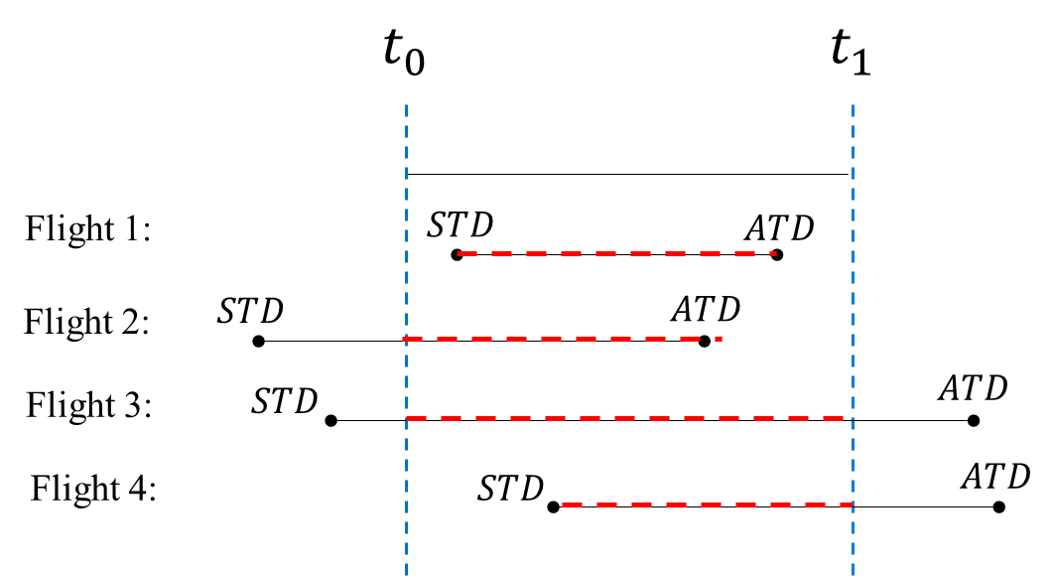
\includegraphics[width=\textwidth]{img/delay decompose.png}
    \caption{Decomposition of departure delay into time slice}
\end{figure}

In this project, the airport connections are identified based on departure delay patterns. We first construct the daily departure delay time series matrix, as illustrated in \hyperref[fig:delay matrices]{fig:delay matrices}.  Each airport has a 3 by 96 matrix. 96 represents the number of 15 min time slice of each day. Each column vector contains the 5th, 50th and 95th percentile of flight departure delay within the time slice. Each row vector is the time series of each delay statistics. The arrival delay matrices are constructed in the same way. 
\begin{figure}[thbp]
    \label{fig:delay matrices}
    \centering
    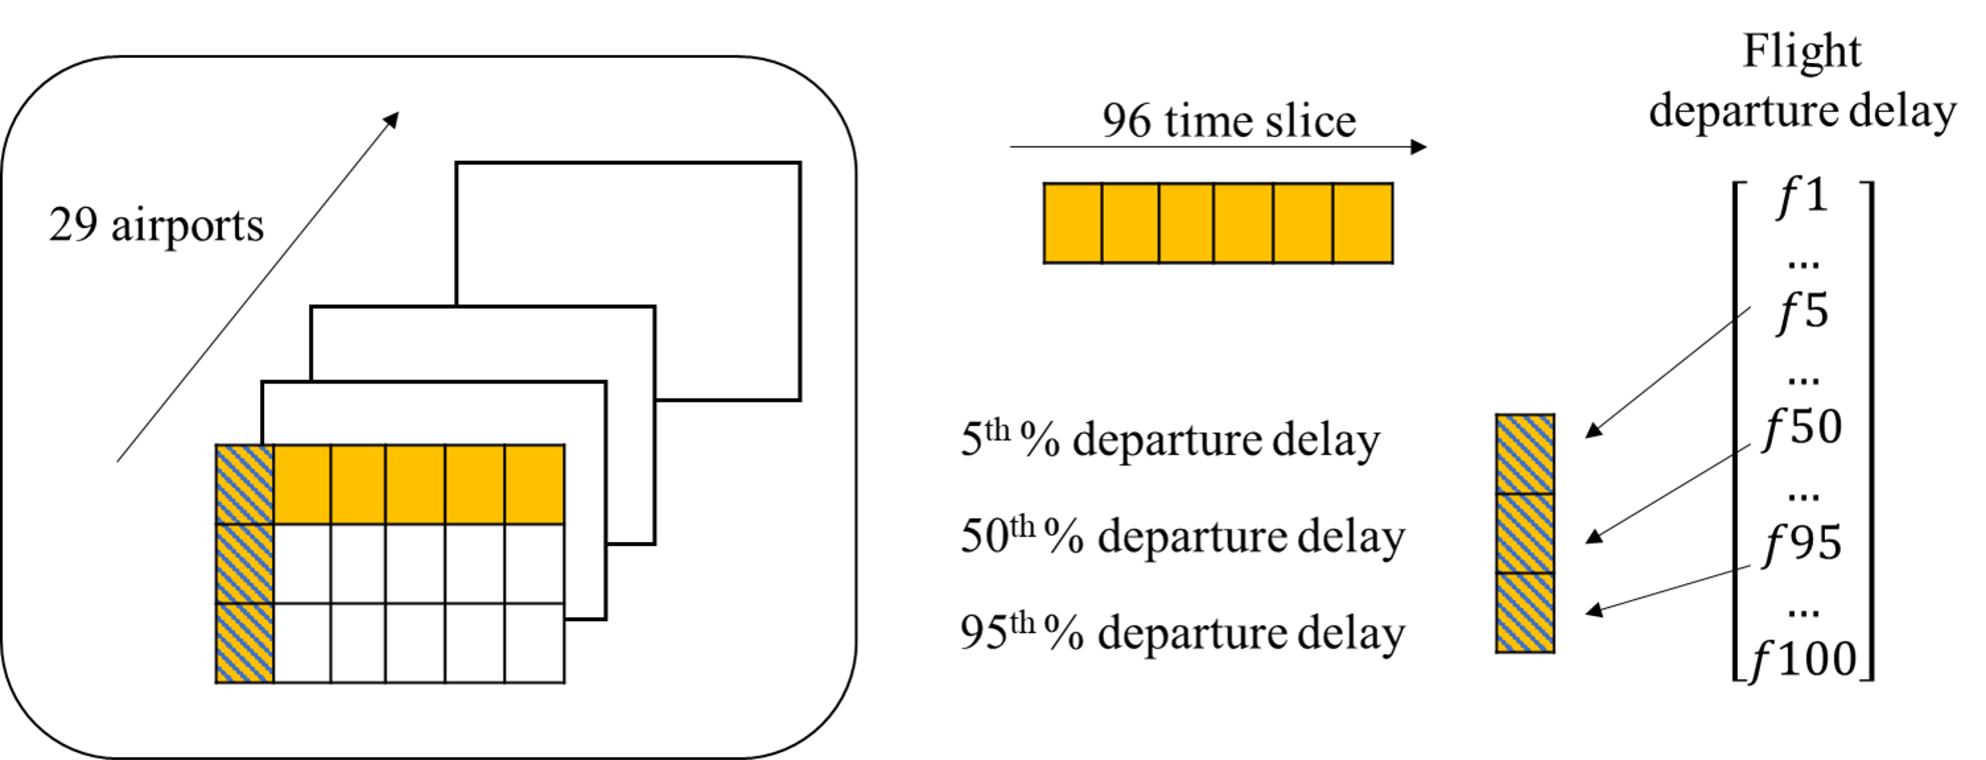
\includegraphics[width=\textwidth]{img/delay matrices.png}
    \caption{Illustration of delay matrices}
\end{figure}

Besides, we also include flight accumulation within each time step as additional features for each airport node. We construct queuing diagram for each airport, as shown in \hyperref[fig:accumulation matrix]{fig:accumulation matrix}. Then the excess accumulation at each time can be calculated by $\mathrm{E(t)}=\mathrm{S(t)}-\mathrm{A(t)}$, where $\mathrm{S(t)}$ is the scheduled cumulative departure, $\mathrm{A(t)}$ actual cumulative departure.

\begin{figure}[thbp]
    \label{fig:accumulation matrix}
    \centering
    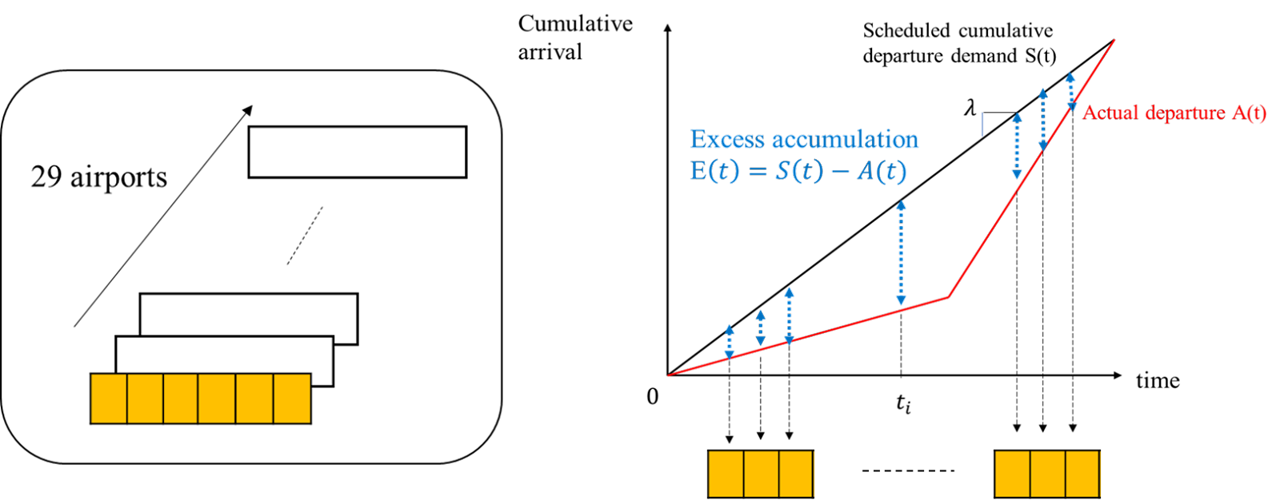
\includegraphics[width=\textwidth]{img/accumulation matrix.png}
    \caption{Illustration of accumulation matrix}
\end{figure}


%Introduction of the dataset
%Preprocess procedure
    %What features? how to generate? Why?

\section{Adaptive Deep Modularity Network (ADMoN)}

The overall framework of the adaptive deep modularity network (ADMoN) is shown in \hyperref[fig:3-1]{Figure 3.1}. As mentioned in the previous section, airport quarter delays of a single day pass a processing pipeline and generate ordered vectors. We initialize the graph structure by using a delay vector to represent the delay feature of an airport and randomly generate an adjacency matrix with each of its elements randomly sampled from a uniform distribution $U(-\frac{1}{\sqrt{n}},\frac{1}{\sqrt{n}})$. The training process of ADMoN consists of jointly optimizing two tasks: graph learning and soft clustering.

\begin{figure}[thbp]
    \label{fig:3-1}
    \centering
    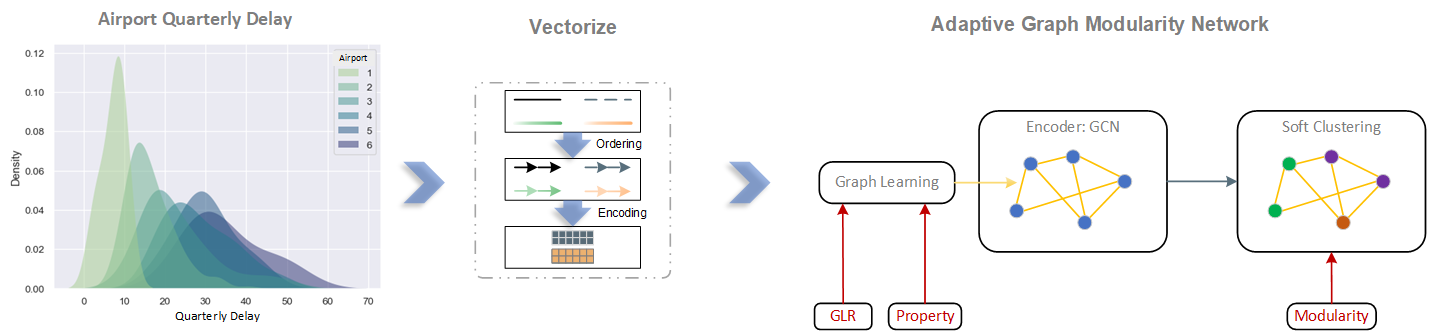
\includegraphics[width=\textwidth]{img/admon.png}
    \caption{Framework of Adaptive Deep Modularity Network}
\end{figure}

\subsection{Graph Learning}

Since the similarity of airport aggregate delay patterns are not readily available, manually construct the relationships can be sub-optimal, we implement data-driven method to extrapolate underlying relationships directly from the delay features obtained. \citet{9102726} proposed a graph learning algorithm exploiting the optimization of the adjacency matrix for both data and tasks. In our implementation, we extend its original real-value node embedding to vector embedding.

To begin with, we expect the optimal adjacency matrix to promote smoothness in graph signal, that is, edges connecting two similar nodes should be associated with higher weights than those connecting dissimilar nodes. In practice, this property can be measure by the \emph{graph Laplacian regularizer} (GLR). Define the combinatorial graph Laplacian matrix by the difference of degree matrix and adjancency matrix\citep{chung1997spectral}:
\begin{equation}
    L=D-A
\end{equation}
where the degree matrix $D$ is a diagonal matrix with its diagonal elements $d_{i,i}=\sum_{j=1}^n a_{i,j}$. Then a graph signal $\mathcal{V}\in\mathbb{R}^{n\times d}$ given on a graph $\mathcal{G}=(\mathcal{V},\tilde{A})$ is \emph{smooth} if
\begin{equation}
    \text{GLR}(\mathcal{V},\tilde{A})=\mathcal{V}^\intercal L\mathcal{V}=\mathcal{V}^\intercal\left(I-\tilde{A}\right)\mathcal{V}
\end{equation}
where $\tilde{A}$ is a normalized adjacency matrix for numerical stability of the model.
\begin{equation}
    \tilde{A}=D^{-\frac{1}{2}}AD^{-\frac{1}{2}}
\end{equation}
We integrate the GLR as a component of the total loss function weighed by $\lambda_0$ for training
\begin{equation}
    \mathcal{L}_{\text{GLR}}=\lambda_0\left\|\mathcal{V}^\intercal\left(I-\tilde{A}\right)\mathcal{V}\right\|_2^2
\end{equation}
Except for the above GLR loss, the learn-able adjacency matrix should satisfy multiple property constraints, including sparsity, symmetric, normalized, and looplessness. Similarly, we integrate them by constructing associated loss functions and assign different weights:
\begin{itemize}
    \item \textbf{Sparsity}. We promote sparse connections to enforce our model capturing only the prominent similarities. Mathematically, we use $l_1$-trick to reduce cardinality of the adjacency matrix:
    \begin{equation}
        \mathcal{L}_{\text{card}}=\lambda_1\|\tilde{A}\|_1
    \end{equation}
    \item \textbf{Symmetric}. As discussed in the previous section, we consider mutual impacts within the network and model the connections as a undirected graph. Therefore, we enforce the learned adjacency matrix to be symmetric:
    \begin{equation}
        \mathcal{L}_{\text{symmetric}}=\lambda_2\left\|\tilde{A}^\intercal-\tilde{A}\right\|_F^2
    \end{equation}
    \item \textbf{Normalized}. For stability, we enforce the learned adjacency matrix normalized:
    \begin{equation}
        \mathcal{L}_{\text{norm}}=\lambda_3\left\|\tilde{A}\textbf{1}-\textbf{1}\right\|_F^2
    \end{equation}
    where $\textbf{1}\in\mathbb{R}^n$ is a vector with all the elements equal to one.
    \item \textbf{Looplessness}. In a airport delay similarity network, it's unnecessary to link a airport with itself. Mathematically, we want the trace of the adjacency matrix to be zero:
    \begin{equation}
        \mathcal{L}_{\text{looplessness}}=\lambda_4\left|\mathbf{tr}(\tilde{A})\right|^2
    \end{equation}
\end{itemize}
With all the above settings, the graph learning process can be expressed as an optimization problem that minimize the following objective function:
\begin{equation}
    \min_{\tilde{A}} \lambda_0\left\|\mathcal{V}^\intercal\left(I-\tilde{A}\right)\mathcal{V}\right\|_2^2+\lambda_1\|\tilde{A}\|_1+\lambda_2\left\|\tilde{A}^\intercal-\tilde{A}\right\|_F^2+\lambda_3\left\|\tilde{A}\textbf{1}-\textbf{1}\right\|_F^2+\lambda_4\left|\mathbf{tr}(\tilde{A})\right|^2
\end{equation}
In this formation, we can manually tune the values of all the weights $\lambda_i,i=0,\ldots,4$ to address different property importance.

\subsection{Airport Soft Clustering}

Based on graph learning, we can directly identify latent structure of the airports by their delay patterns. Since the GLR leads to an inhomogeneous distribution of edge weights, we can infer \emph{clusters} (also known by \emph{communities} or \emph{modules}) consisting of airports with high intra-cluster weight density and low inter-cluster density. \citet{tsitsulin2020graph} proposed a Deep Modularity Network (DMoN) model which is driven by the modularity measure of clustering quality. It simultaneously learn the graph embedding and proper cluster assignments of the nodes. They use a graph convolutional neural network (GCN) \citep{https://doi.org/10.48550/arxiv.1609.02907} combined with skip connection as the kernel transformation function.
\begin{equation}
    \mathcal{K}(\mathcal{V},\tilde{A})=\text{GCN}(\mathcal{V},\tilde{A})=\tilde{A}\mathcal{V}W+\mathcal{V}W_{\text{skip}}
\end{equation}
where both $W$ and $W_{\text{skip}}$ are learn-able weight matrices that project features from high-dimensional metric space into a low-dimensional hidden space. The model is trained on an objective to maximize the spectral modularity (i.e., the measure of network division strength) and penalize assigning all the nodes into the same cluster (i.e., a collapse regularization term). The objective problem is as follows:
\begin{equation}
    \min_{W,W_{\text{skip}}}-\frac{1}{2m}\mathbf{tr}(C^\intercal AC-C^\intercal d^\intercal dC)+\frac{\sqrt{K}}{n}\left\|\sum_iC_i^\intercal\right\|_F-1: C=\text{Softmax}(\tilde{A}\mathcal{V}W+\mathcal{V}W_{\text{skip}})
\end{equation}
where $C\in\mathbb{R}^{n\times K}$ is the soft cluster results of the graph with each element $c_{ik}$ the probability of node $i$ as a member of cluster $k$, $d$ is the degree vector of all the nodes, and $m$ the number of edges. We propose to combine graph learning with DMoN to allow adaptive graph structure inference and name it Adaptive Deep Modularity Network (ADMoN).

We use "warm-up and fine-tune" strategy for training. At first, we use batches of aggregate delay features with back propagation to train the model and derive a warm-up parameter estimation. Then, we further fine-tune our model using single batch of data and obtain final adjacency matrix and cluster assignments regarding each batch of data.

\subsection{Extension: Daily Connection Identification}
\label{ch_3_3_3}

As shown in \hyperref[fig:3-2]{Figure 3.2}, if the input aggregated delay features are daily based, we can estimate the airport connections with respect to each day as adjacency matrix $A_i$. Since eigenvalues of a adjacency matrix has proven to be a useful graph features for machine learning tasks \cite{schmidt2014spectral}, we use eigenvalues of adjacency matrices to construct the node feature matrix $\mathcal{V}^\prime$ in daily connection graph.
\begin{equation}
    v_i^\prime=SP(\tilde{A})=\text{diag}(\Lambda):\tilde{A}Q=Q\Lambda, v_i^\prime\in\mathcal{V}^\prime
\end{equation}
where $\tilde{A}Q=Q\Lambda$ is the spectral decomposition of normalized adjacency matrix $\tilde{A}$. By injecting the new graph into ADMoN framework, we can identify latent connections among operational days based on airport delay connection patterns.

\begin{figure}[thbp]
    \label{fig:3-2}
    \centering
    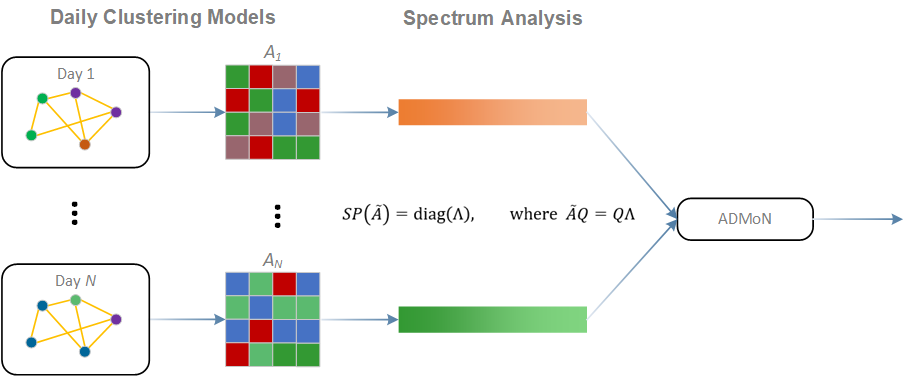
\includegraphics[width=\textwidth]{img/extension.png}
    \caption{Extension of ADMoN on inferring operational day connection}
\end{figure}

% \begin{tcolorbox}[breakable,title={An example colorbox},
% colback=founderblue!5!white,
% colframe=founderblue!75!black,
% fonttitle=\headingfont\bfseries\large]
% Your text goes here. The colors are based on Berkeley's Founder Blue.
% \tcbsubtitle[before skip=\baselineskip]%
% {You can also have subboxes}
% Don't like the colors? You can change them here (replace founderblue with the color you like), or you can change them globally in the colors section of report.tex
% \tcbsubtitle[before skip=\baselineskip]%
% {Multiple rows}
% If you like it.

% \end{tcolorbox}






